\documentclass[aspectratio=169,handout]{beamer}
\usetheme{boxes}
\usefonttheme{professionalfonts,structurebold}
\usecolortheme{dove}

\usepackage[advantage,asymptotics,adversary,sets,keys,ff,lambda,primitives,events,operators,probability,logic,mm,complexity]{cryptocode}
\usepackage[capitalise]{cleveref}
\usepackage{scrextend}
\changefontsizes{9pt}

\usepackage{tikz}
\usetikzlibrary{positioning,arrows}

\title{Non malleability of the Fiat-Shamir transformation}
\author{\normalsize{Michal Zajac \inst{1} \and Markulf Kohlweiss \inst{2}}}
\institute{\inst{1} Clearmatics \inst{2}IOHK}
\date{}

\newcommand{\newdefs}[1] {\setlength{\fboxsep}{1pt}\colorbox{gray!20}{\(#1\)}}

\newcommand{\COMMENT}[1]  {}

%general formatting
\newcommand{\pcvarstyle}[1]{\mathsf{#1}}
\newcommand{\comment}[1]{{\color{lightgray}#1}}

% General mathematics
\newcommand{\range}[2] {[#1 \, .. \, #2]}
\newcommand{\SD}{\Delta}
\newcommand{\smallset}[1] {\{#1\}}
\newcommand{\bigset}[1] {\left\{#1\right\}}
\newcommand{\GRP} {\mathbb{G}}
\newcommand{\pair} {\hat{e}}
\newcommand{\brak}[1] {\left(#1\right)}
\newcommand{\sbrak}[1] {(#1)}
\newcommand{\alg}[1] {\pcalgostyle{#1}}
\newcommand{\image} {\operatorname{im}}
\newcommand{\myland} {\,\land\,}
\newcommand{\mylor} {\,\lor\,}
\newcommand{\vect}[1] {\operatorname{vect}(#1)}
\newcommand{\w}{\omega}
\newcommand{\const}{\pcpolynomialstyle{const}}

% bilinear maps

\newcommand{\bmap}[2] {\left[#1\right]_{#2}}
\newcommand{\gone}[1] {\bmap{#1}{1}}
\newcommand{\gtwo}[1] {\bmap{#1}{2}}
\newcommand{\gi} {\iota}
\newcommand{\gtar}[1] {\bmap{#1}{T}}
\newcommand{\grpgi}[1] {\bmap{#1}{\gi}}


% zero knowledge
\newcommand{\oracleo}{\mathsf{O}}
\newcommand{\crs}{\pcvarstyle{crs}}
\newcommand{\td}{\pcvarstyle{td}}
\newcommand{\ip}[2]{\left\langle #1, #2\vphantom{A^B}\right\rangle}
\newcommand{\zkproof}{\pi}
\newcommand{\proofsystem}{\mathrm{\Psi}}
\newcommand{\nuppt}{\pcmachinemodelstyle{NUPPT}}
\newcommand{\ro}{\mathcal{H}}
\newcommand{\trans}{\pcvarstyle{trans}}
\newcommand{\tr}{\pcvarstyle{tr}}
\newcommand{\instsize}{\pcvarstyle{n}}
\newcommand{\KG} {\mathsf{K}}
\newcommand{\kcrs} {\KG_{\crs}}
\renewcommand{\dist}{\ddv}

% general complexity theory
\newcommand{\RND}[1]{\pcalgostyle{RND}(#1)}
\newcommand{\RELGEN}{\mathcal{R}}
\newcommand{\REL}{\mathbf{R}}
\newcommand{\LANG}{\mathcal{L}}
\newcommand{\inp}{\pcvarstyle{x}}
\newcommand{\wit}{\pcvarstyle{w}}
\newcommand{\class}[1]{\mathfrak{#1}}
\newcommand{\ig}{\pcalgostyle{IG}}
\newcommand{\accProb}{\event{acc}}
\newcommand{\extProb}{\event{ext}}
\newcommand{\FS}{\pcalgostyle{FS}} % Fiat-Shamir transform
\newcommand{\aux}{\pcvarstyle{aux}} %auxiliary input

%Plonk and Sonic
\newcommand{\plonk}{\textsc{Plonk}}
\newcommand{\sonic}{\textsc{Sonic}}
\newcommand{\maxdegree}{\pcvarstyle{N}}

\newcommand{\iur}{i\text{-}\mathsf{UR}}

%colors
\definecolor{darkmagenta}{rgb}{0.5,0,0.5}
\definecolor{lightmagenta}{rgb}{1,0.85,1}
\definecolor{lightmagenta}{rgb}{0.9,0.9,0.9}
\definecolor{darkred}{rgb}{0.7,0,0}
\definecolor{blueish}{rgb}{0.1,0.1,0.5}
\definecolor{pinkish}{rgb}{0.9,0.8,0.8}
\definecolor{darkgreen}{rgb}{0,0.6,0}
\definecolor{lightgreen}{rgb}{0.85,1,0.85}
\definecolor{skyblue}{rgb}{0.3,0.9,0.99}

%coments
\DeclareRobustCommand{\michals}[2]  {{\color{blueish}\sethlcolor{pinkish}\hl{\scriptsize\textsf{Michal #1:} #2}}}
\newcommand{\task}[2]{\todo[author=\textbf{Task},inline]{({\textit{#1}}) #2}}
% \newcommand{\task}[2] {\xcommenti{Task}{#1}{#2}}
% \DeclareRobustCommand{\task}[2]  {{\color{black}\sethlcolor{yellow}\hl{\textsf{TASK #1:} #2}}}

\renewcommand{\emph}[1]{\textbf{#1}}

\newcommand{\advfs}{\adv_\fs}
\renewcommand{\myskip}{0.5\baselineskip}

\begin{document}

\begin{frame}
\titlepage
\end{frame}

\begin{frame}
  \frametitle{Our result}
  \begin{center}
    \fbox{\parbox{10cm}{\centering We show that a class (for example $\plonk$, $\sonic$)
        of RO-based NIZKs is \emph{simulation extractable} }}
  \end{center}

  \begin{block}{Simulation extractability}
    \begin{columns}
      \begin{column}{0.5\linewidth}
    Adversary $\adv$ is given oracle access to a simulator $\simulator$, can
    query it on instances $\inp$ and get a simulated proof $\zkproof$.\\[\myskip]
    Eventually, $\adv$ outputs instance and proof $\inp', \zkproof'$.\\[\myskip]
    We say that proof system $\PS$ is \emph{simulation extractable} if there exists an
    extractor $\ext$ that given $\adv$ and its randomness outputs $\wit'$ such that
    $\REL(\inp', \wit')$
  \end{column}
  \begin{column}{.4\linewidth}
    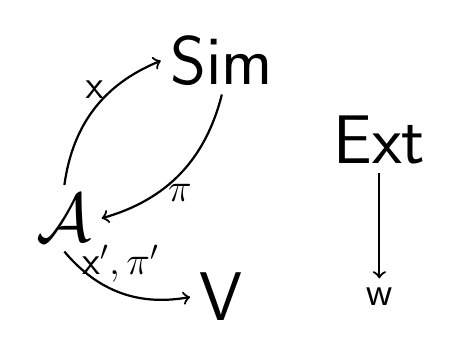
\begin{tikzpicture}
      \draw (0, 0) node (adv) {\Huge $\adv$};
      \draw (2, 2) node (sim) {\Huge
        $\simulator$};
      \draw (2, -1) node (ver) {\Huge $\verifier$}; 
      \draw[thick,->] (adv.north) to [bend left] node[anchor=south]
      {\Large$\inp$} (sim.west);
      \draw[thick,->] (sim.south) to [bend left] node[anchor=north]
      {\Large$\zkproof$} (adv.east);
      \draw[thick,->] (adv.south) to [bend right] node[anchor=south]
      {\Large{$\inp',\zkproof'$}} (ver.west);\pause
      \draw (4, 1) node (ext) {\Huge $\ext$};
      \draw (4, -1) node (wit) {\Large $\wit$};
      \draw[thick,->] (ext.south) to (wit.north);
    \end{tikzpicture}
  \end{column}
  \end{columns}
  \end{block}
  
  \begin{block}{Why simulation extractability matters}
    Proofs done in a ``stand-alone'' model don't fit well to the real world\\
    In the real world malicious provers may see multiple proofs and learn from
    them\\
    Not covered by standard soundness / knowledge soundness definition
  \end{block}
\end{frame}

\begin{frame}
  \frametitle{Our result -- ct'd}
  \begin{block}{Example}
  \end{block}
  \begin{block}{Required properties}
    Unique response property\\
    Trapdoor-free simulatability\\
    Generalized general forking lemma
  \end{block}
\end{frame}

\begin{frame}
  \frametitle{}
\end{frame}

\begin{frame}
  % \frametitle{Prior our work}
  \begin{block}{Some background}
    Most efficient \emph{universal} or \emph{updatable} zkSNARKs use random-oracle
  \end{block}\pause  

  \begin{block}{Prior state-of-the-art}
    %\begin{itemize}
    %\item
    Proven security of the \emph{interactive} proof system
    % \item

    Security of the \emph{non-interactive} variant conjectured
      relying on Fiat--Shamir transformation
    %\end{itemize}
  \end{block}\pause

  \begin{block}{Problems}
    Fiat--Shamir transformation relies on \emph{forking lemma}

    Forking lemma shown secure only for a narrow class of protocols
    that \emph{requires only a single rewinding}

    Not a case for any known zkSNARK
  \end{block}\pause

  \begin{block}{The result}
    Generalized Fiat--Shamir transformation to work with wider class of protocols
    
     Shown that a wide class of RO-based zkSNARKs are
     simulation-extractable \emph{out-of-the-box}
     
     This includes: Plonk, Sonic, some variants of Marlin
  \end{block}
\end{frame}

\section{Fiat--Shamir transformation}
\begin{frame}
  \frametitle{$\Sigma$-protocols}
  \begin{columns}
    \begin{column}{.3\linewidth}
      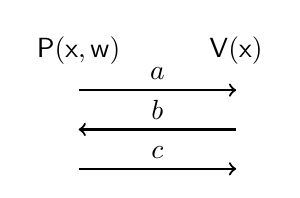
\begin{tikzpicture}
        \draw (0, 0) node (prover) {$\prover(\inp, \wit)$}; \draw (2, 0) node
        (verifier) {$\verifier(\inp)$};

        \draw[thick,->] (0, -0.5) -- node[anchor=south] {$a$} (2, -0.5);

        \draw[thick,->] (2, -1) -- node[anchor=south] {$b$} (0, -1);
        
        \draw[thick,->] (0, -1.5) -- node[anchor=south] {$c$} (2, -1.5);
      \end{tikzpicture}
    \end{column}
    \begin{column}{.6\linewidth}
      \begin{block}{Completeness}
        Honest verifier accepts proof from an honest prover.
      \end{block}
      \begin{block}{Special soundness}
        Given two transcripts for instance $(\inp, a, b, c)$ and
        $(\inp, a, b', c')$ one can compute witness $\wit$.
      \end{block}
      \begin{block}{Honest verifier zero knowledge}
        The protocol is zero-knowledge if the verifier picks its challenges randomly.
      \end{block}
      \begin{block}{Public coin}
        The verifier's challenges are public function of its randomness.
      \end{block}
    \end{column}
  \end{columns}
\end{frame}

\begin{frame}
  \frametitle{$\Sigma$-protocols. Schnorr protocol -- proof of knowledge of a discrete logarithm}
  \begin{columns}
    \begin{column}{.5\linewidth}
      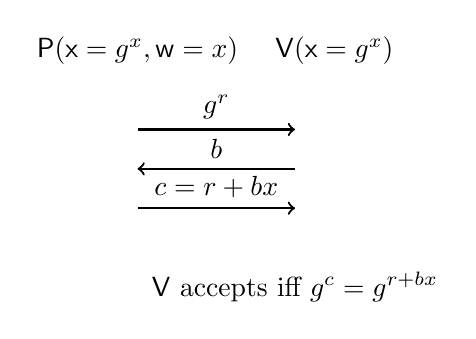
\begin{tikzpicture}
        \draw (0, 0.5) node (prover) {$\prover(\inp = g^x, \wit = x)$};
        \draw (2.5, 0.5) node (verifier) {$\verifier(\inp = g^x)$};
        \draw[thick,->] (0, -0.5) -- node[anchor=south] {$g^r$} (2, -0.5);
        \draw[thick,->] (2, -1) -- node[anchor=south] {$b$} (0, -1);
        \draw[thick,->] (0, -1.5) -- node[anchor=south] {$c = r + bx$} (2, -1.5);
        \draw (2, -2.5) node {$\verifier$ accepts iff $g^c = g^{r+ bx}$};
      \end{tikzpicture}
    \end{column}
    \begin{column}{.5\linewidth}
      \begin{block}{Special soundness}
        From $(g^r, b, r + bx)$ and $(g^r, b', r + b'x)$, one computes
        \[
          r + bx - (r + b'x)  = (b - b')x
        \]
        Hence, for $b \neq b'$ one may reveal $x$.
      \end{block}
    \end{column}
  \end{columns}
\end{frame}

\begin{frame}
  \frametitle{$\Sigma$-protocols -- Fiat--Shamir transformation}
  \begin{columns}
    \begin{column}{.3\linewidth}
      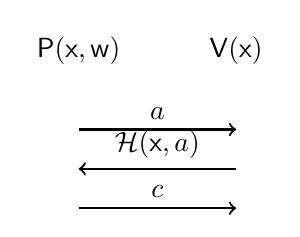
\begin{tikzpicture}
        \draw (0, 0) node (prover) {$\prover(\inp, \wit)$}; \draw (2, 0) node
        (verifier) {$\verifier(\inp)$};
        \draw[thick,->] (0, -1) -- node[anchor=south] {$a$} (2, -1);
        \draw[thick,->] (2, -1.5) -- node[anchor=south] {$\ro(\inp, a)$} (0, -1.5);
        \draw[thick,->] (0, -2) -- node[anchor=south] {$c$} (2, -2);
      \end{tikzpicture}
    \end{column}
    \begin{column}{.6\linewidth}
      \begin{block}{Completeness}
        Honest verifier accepts proof from an honest prover.
      \end{block}
      \begin{block}{Special soundness}
        Given two transcripts for instance $(\inp, a, b, c)$ and $(\inp, a, b',
        c')$ one can compute witness $\wit$.
      \end{block}
      \begin{block}{Honest verifier zero knowledge}
        The protocol is zero-knowledge if the verifier picks its challenges randomly.
      \end{block}
      \fbox{\parbox{5cm}{
      \begin{block}{Public coin}
        The verifier's challenges are public function of its randomness.
      \end{block}
    }}
    \end{column}
  \end{columns}
\end{frame}

\begin{frame}
  \frametitle{Soundness of the Fiat--Shamir transformation}
  \begin{columns}
    \begin{column}{0.5\linewidth}
  \begin{block}{How to get two transcripts from $\advfs$}
    Get one transcript $(\inp, a, b = \ro(\inp, a), c)$.\\
    Rewind $\advfs$ after it sent $a$.\\
    Pick new $\ro$ response $b'$ for $\ro(\inp, a)$.\\
    Get another transcript $(\inp, a, b', c').$
  \end{block}
  
  \begin{block}{Problem}
    $\adv$ has \emph{one shot} to convince the verifier $\verifier$.

    If $\advfs$ does not like $\verifier$'s challenge, it may pick \emph{another}
    instance $\inp$ or $a$ and try again.\\[\myskip]
    What if the adversary keeps changing the instance so we cannot get $2$
    transcripts?\\[\myskip]
    What is the probability that we obtain two acceptable transcripts $(\inp, a,
    b, c)$ and $(\inp, a, b', c')$?
    % The reduction needs to \emph{guess} which random oracle call is going to be
    % used in the final proof.\\
    % If $\advfs$ makes $Q$ queries, this probability is $\frac{1}{Q}$.
  \end{block}


% \iffalse
%   \begin{block}{Proof overview}
%     Assume $\PS$ is sound. We show that $\PS_\fs$ is sound as well.\\[\myskip]
%     Reduction $\rdv$ internally runs $\advfs$ and talks to $\PS.\verifier$.\\
%     If $\advfs$ is successful in breaking soundness of $\PS_\fs$, then $\rdv$ is
%     successful in breaking soundness of $\PS$.
%   \end{block}
% \fi
\end{column}
\begin{column}{0.5\linewidth}
  \begin{block}{Forking lemma}
    Let $\accProb$ be a probability that $\advfs$ returns an acceptable proof.\\
    $q$ -- upper bound for a number of random oracle queries $\advfs$ may
    make.\\
    $h$ -- range size of the random oracle.
    \[
      \frkProb \geq \accProb \left(\frac{\accProb}{q} - \frac{1}{h}\right).
    \]
  \end{block}
    % \begin{tikzpicture}
  %   \draw (0, 0) node (reduction) {$\rdv$};
  %   \draw (2, 0) node 
  %   (verifier) {$\verifier(\inp)$}; \draw[thick,->] (0, -1) --
  %   node[anchor=south] {$a$} (2, -1); \draw[thick,->] (2, -2) --
  %   node[anchor=south] {$b$} (0, -2); \draw[thick,->] (0, -3) --
  %   node[anchor=south] {$c$} (2, -3);
  % \end{tikzpicture}
\end{column}
\end{columns}
\vspace*{0.5cm}
\centering\fbox{\parbox{10cm}{\centering What if there is more than just mere $2$
    rounds?\\
    What if there is more than just mere $2$ transcripts are
  necessary?}}
\end{frame}

% \begin{frame}
  
% \end{frame}

\begin{frame}
  \frametitle{Simulation-extractability of $\Sigma$-protocols}
  \begin{center}{\fbox{Let
      $\Psi_\fs$ be a Fiat--Shamir transformed $\Sigma$-protocol $\Psi$. Then
      $\Psi_\fs$ is simulation-extractable}}
\end{center}
\begin{columns}
  \begin{column}{.4\linewidth}
  \begin{block}{Caveats}
    The protocol $\Psi$ has to have \emph{unique response property}\\
    Simulation extractability depends on the probability $\accProb$
  \end{block}
\end{column}
\begin{column}{.4\linewidth}
  \begin{block}{Unique response property}
    $\Psi$ has unique response property if no $\ppt$ adversary $\adv$ can come
    up with two acceptable transcripts\\
    $(\inp, a, b, c)$ and $(\inp, a, b, c')$.
  \end{block}
\end{column}
\end{columns}
\end{frame}

\begin{frame}
  \frametitle{Generalized forking lemma}
  \begin{columns}
    \begin{column}{.4\linewidth}
  \begin{block}{Pros}
    Covers case of \emph{multiround protocols}\\
    Fine with protocols that require more than $2$ transcripts to reveal the witness
  \end{block}
  
  \begin{block}{Cons}
    Huge number of rewinds required to reveal the witness\\
    (Probably inevitable)
  \end{block}

  \begin{block}{Probability of successful forking}
    $\accProb$ -- probability that $\advfs$ outputs an acceptable proof\\
    $q$ -- number of random oracle queries that $\advfs$ makes\\
    $h$ -- size of the random oracle range\\
    $m$ -- number of necessary rewinds to reconstruct the witness
    \[
      \frac{\accProb}{q^{m - 1}} - \accProb \left(1 - \frac{h!}{h - m}! \cdot
        h^m\right)
    \]
  \end{block}
\end{column}
\begin{column}{.4\linewidth}
  \begin{block}{$(n_1, \ldots, n_k)$-tree}
    Is a tree where every node on depth $i$ has $n_i - 1$ siblings and
    $n_{i + 1}$ children. (In total $\prod_{i = 1}^k n_i$ paths)
  \end{block}
  \begin{block}{Tree of acceptable transcripts}
    Consider a $(n_1, \ldots, n_k)$-tree. Let nodes be prover's messages and
    edges between them verifier's challenges. 
  \end{block}
\end{column}
\end{columns}
\end{frame}

\begin{frame}
  \frametitle{}
\end{frame}

\begin{frame}
  \frametitle{Security of FS transformation---forking lemma}
  \begin{lemma}[General forking lemma, cf.~\cite{INDOCRYPT:FKMV12,CCS:BelNev06}]
    \label{lem:forking_lemma}
    \begin{columns}
      \begin{column}{.5\linewidth}
	Fix $q \in \ZZ$ and a set $H$ of size $h > 2$. Let $\zdv$ be a $\ppt$
  algorithm that on input $y, h_1, \ldots, h_q$ returns $(i, s)$, where $i
  \in\range{0}{q}$ and $s$ is called a \emph{side output}. Denote by $\ig$ a
  randomised instance generator. We denote by $\accProb$ the probability
	\[
		\condprob{i > 0}{y \gets \ig; h_1, \ldots, h_q \sample H; (i, s) \gets
		\zdv(y, h_1, \ldots, h_q)}\,.
	\]
	Let $\forking_\zdv(y)$ denote the algorithm described in
  \cref{fig:forking_lemma}, then the probability $\frkProb$ defined as $
  \frkProb := \condprob{b = 1}{y \gets \ig; (b, s, s') \gets \forking_{\zdv}(y)}
  $ holds
	\[
		\frkProb \geq \accProb \brak{\frac{\accProb}{q} - \frac{1}{h}}\,.
	\]
      \end{column}
      \begin{column}{.4\linewidth}
	\begin{figure}
		\centering
		\fbox{
		\procedure{$\forking_\zdv (y)$}
		{
			\rho \sample \RND{\zdv}\\
			h_1, \ldots, h_q \sample H\\
			(i, s) \gets \zdv(y, h_1, \ldots, h_q; \rho)\\
			\pcif i = 0\ \pcreturn (0, \bot, \bot)\\
			h'_{i}, \ldots, h'_{q} \sample H\\
			(i', s') \gets \zdv(y, h_1, \ldots, h_{i - 1}, h'_{i}, \ldots,  h'_{q};
			\rho)\\
			\pcif (i = i') \land (h_{i} \neq h'_{i})\ \pcreturn (1, s, s')\\
			\pcind \pcelse \pcreturn (0, \bot, \bot)
		}}
		\caption{Forking algorithm $\forking_\zdv$}
		\label{fig:forking_lemma}
              \end{figure}
            \end{column}
            \end{columns}
\end{lemma}

\end{frame}

\end{document}